% ============================================
% CHƯƠNG 4: HIỆN THỰC
% ============================================

\section{Hiện thực}

Chương này trình bày chi tiết các trang và tính năng đã xây dựng trong dự án, kèm theo hình ảnh minh họa.

% ------------------------------------------
\subsection{Giao diện trang chủ}

Trang chủ là điểm tiếp xúc đầu tiên với người dùng, được thiết kế với bố cục rõ ràng và hấp dẫn.

\textbf{Các thành phần chính:}
\begin{itemize}
    \item \textbf{Header:} Logo, thanh tìm kiếm, navigation menu, icon giỏ hàng và tài khoản
    \item \textbf{Banner:} Slider quảng cáo sản phẩm nổi bật
    \item \textbf{Featured Products:} Grid hiển thị sản phẩm được đề xuất
    \item \textbf{Categories:} Danh mục sách theo thể loại
    \item \textbf{Footer:} Thông tin liên hệ, links, social media
\end{itemize}

\begin{figure}[H]
\centering
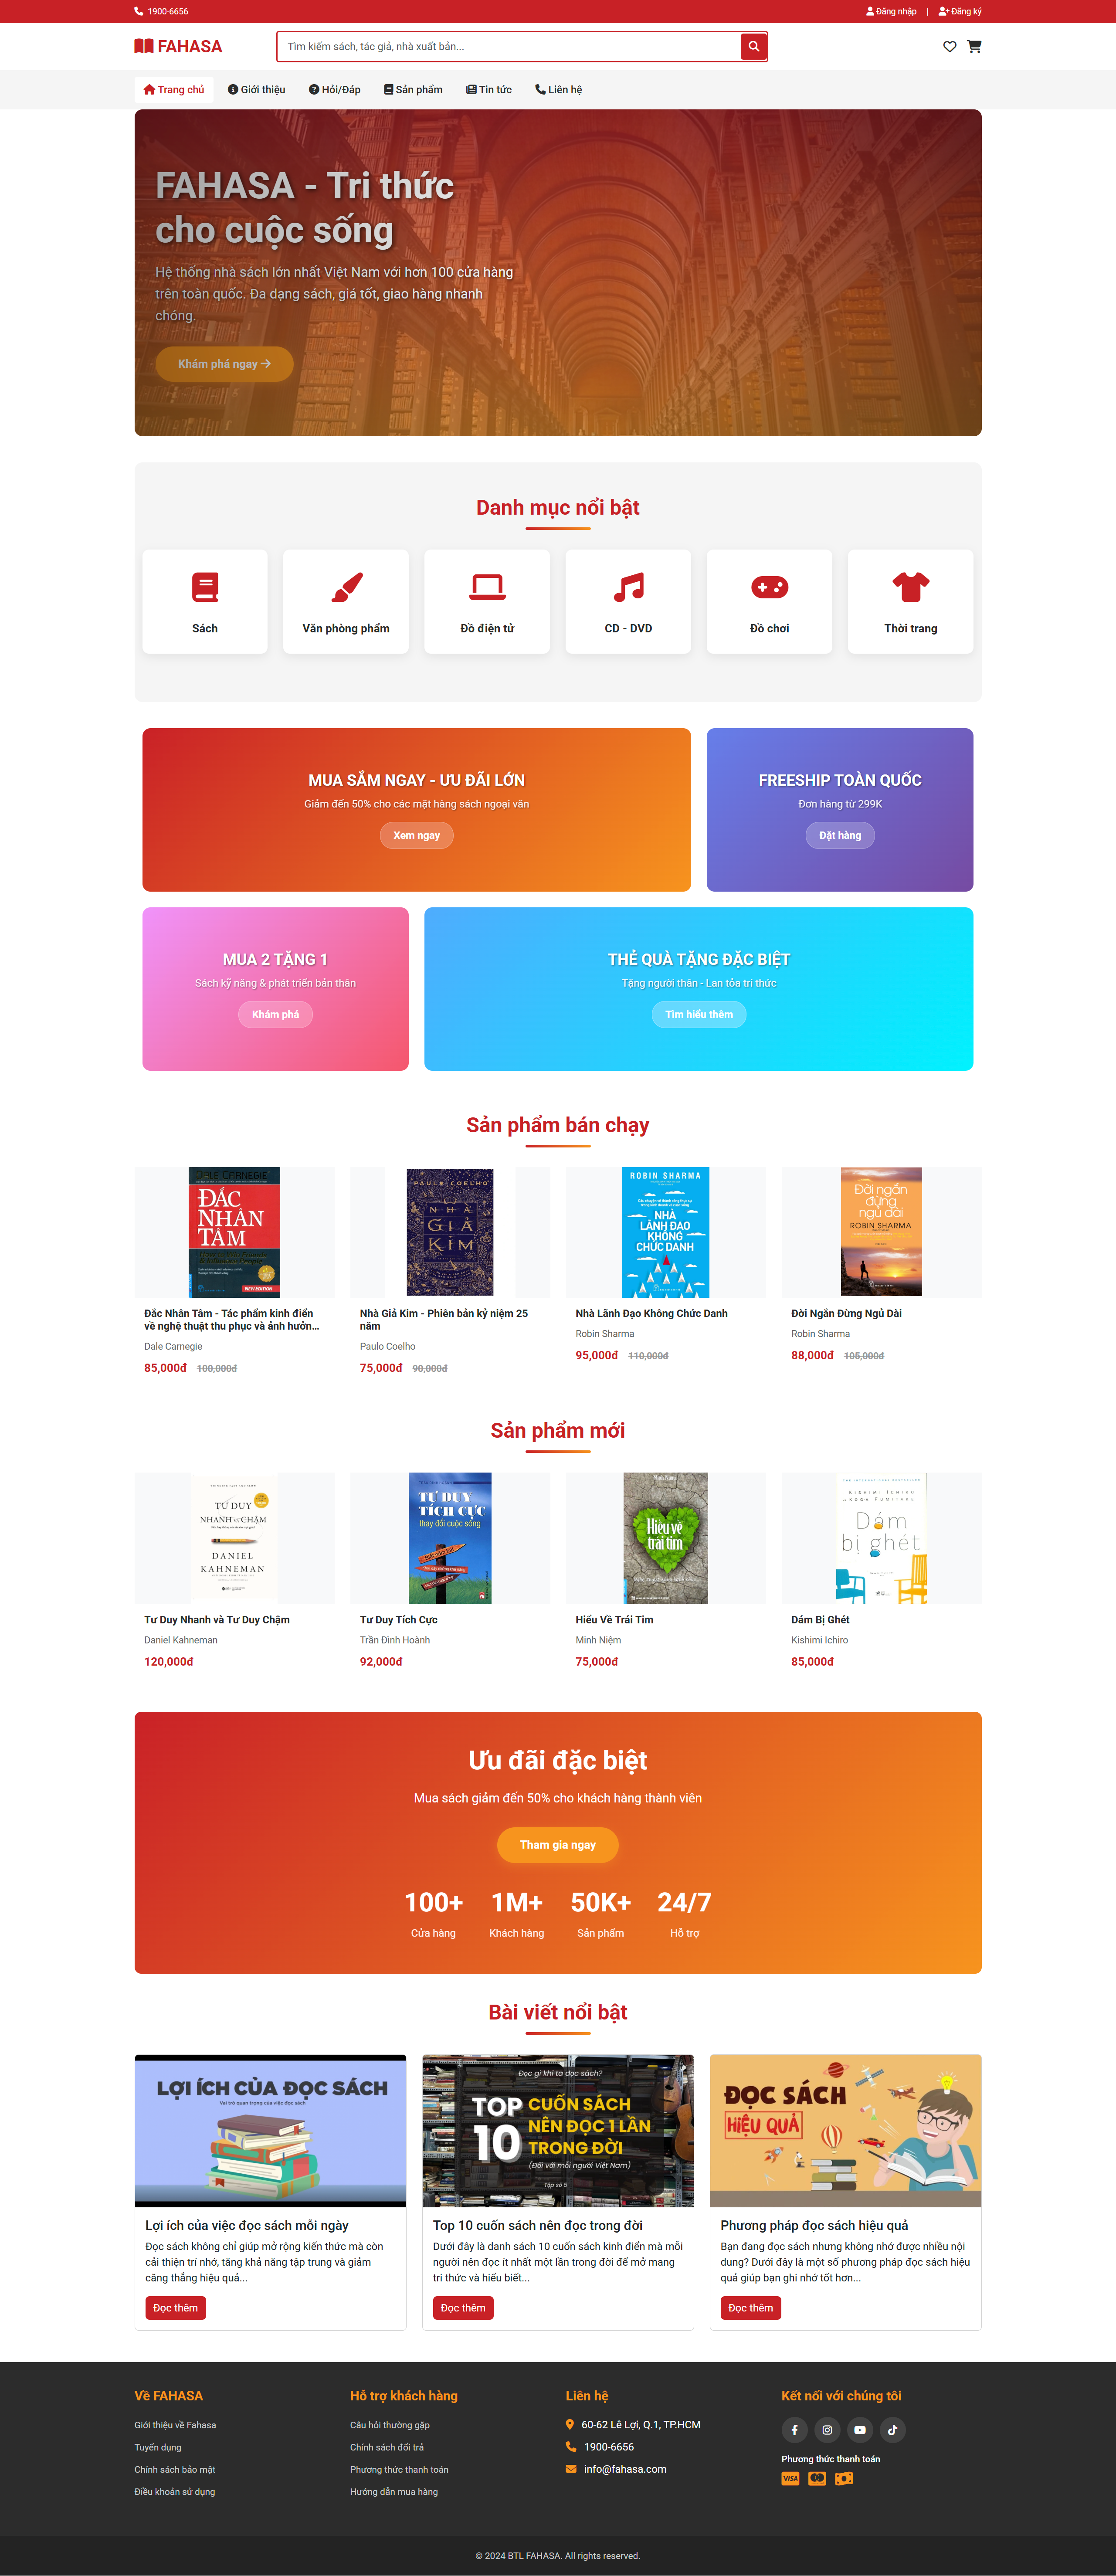
\includegraphics[width=0.6\textwidth]{Images/home_page.png}
\caption{Giao diện trang chủ Fahasa Clone}
\label{fig:home}
\end{figure}

% ------------------------------------------
\subsection{Trang sản phẩm}

\subsubsection{Danh sách sản phẩm}

Trang danh sách hiển thị tất cả sản phẩm với các tính năng:
\begin{itemize}
    \item Grid layout responsive (4 cột desktop, 2 cột mobile)
    \item Card sản phẩm với hình ảnh, tên, giá, badge giảm giá
    \item Lọc theo danh mục
    \item Sắp xếp theo giá, tên, newest
    \item Pagination
\end{itemize}

\begin{figure}[H]
\centering
\includegraphics[width=0.6\textwidth]{Images/product_list.png}
\caption{Trang danh sách sản phẩm}
\label{fig:product-list}
\end{figure}

\subsubsection{Chi tiết sản phẩm}

Trang chi tiết cung cấp thông tin đầy đủ về một sản phẩm:
\begin{itemize}
    \item Hình ảnh sản phẩm lớn, có thể zoom
    \item Thông tin: tên, tác giả, giá gốc, giá khuyến mãi
    \item Mô tả chi tiết sản phẩm
    \item Nút "Thêm vào giỏ" và "Mua ngay"
    \item Sản phẩm liên quan
\end{itemize}

\begin{figure}[H]
\centering
\includegraphics[width=0.6\textwidth]{Images/product_detail.png}
\caption{Trang chi tiết sản phẩm}
\label{fig:product-detail}
\end{figure}

% ------------------------------------------
\subsection{Giỏ hàng}

Tính năng giỏ hàng cho phép người dùng quản lý các sản phẩm đã chọn mua.

\textbf{Các chức năng:}
\begin{itemize}
    \item Xem danh sách sản phẩm trong giỏ
    \item Tăng/giảm số lượng với nút +/-
    \item Xóa sản phẩm khỏi giỏ
    \item Tính toán tự động tổng tiền
    \item Hiển thị số lượng sản phẩm trên icon giỏ hàng
\end{itemize}

\begin{figure}[H]
\centering
\includegraphics[width=0.7\textwidth]{Images/cart_page.png}
\caption{Trang giỏ hàng}
\label{fig:cart}
\end{figure}

\textbf{Xử lý phía server:}

CartController xử lý các action:
\begin{itemize}
    \item \texttt{index()}: Hiển thị giỏ hàng
    \item \texttt{add()}: Thêm sản phẩm
    \item \texttt{update()}: Cập nhật số lượng
    \item \texttt{remove()}: Xóa sản phẩm
\end{itemize}

Giỏ hàng được lưu trong \texttt{\$\_SESSION['cart']} dưới dạng array.

% ------------------------------------------
\subsection{Trang khách hàng}

\subsubsection{Thông tin tài khoản}

Cho phép người dùng xem và chỉnh sửa thông tin cá nhân:
\begin{itemize}
    \item Họ tên, email, số điện thoại
    \item Giới tính, ngày sinh
    \item Địa chỉ giao hàng
\end{itemize}

\begin{figure}[H]
\centering
\includegraphics[width=0.7\textwidth]{Images/customer_profile.png}
\caption{Trang thông tin tài khoản}
\label{fig:profile}
\end{figure}

\subsubsection{Đơn hàng của tôi}

Hiển thị lịch sử đơn hàng với các filter:
\begin{itemize}
    \item Tất cả đơn hàng
    \item Đang xử lý
    \item Đang giao
    \item Hoàn thành
    \item Đã hủy
\end{itemize}

\begin{figure}[H]
\centering
\includegraphics[width=0.7\textwidth]{Images/my_order.png}
\caption{Trang đơn hàng của tôi}
\label{fig:orders}
\end{figure}

\subsubsection{Thông báo}

Hiển thị các thông báo hệ thống về đơn hàng, khuyến mãi:

\begin{figure}[H]
\centering
\includegraphics[width=0.7\textwidth]{Images/notifications.png}
\caption{Trang thông báo}
\label{fig:notifications}
\end{figure}

\subsubsection{Sản phẩm yêu thích}

Danh sách các sản phẩm được đánh dấu yêu thích:

\begin{figure}[H]
\centering
\includegraphics[width=0.7\textwidth]{Images/wishlist.png}
\caption{Trang sản phẩm yêu thích}
\label{fig:wishlist}
\end{figure}

% ------------------------------------------
\subsection{Trang tin tức}

\subsubsection{Danh sách bài viết}

Hiển thị các bài viết, tin tức về sách:

\begin{figure}[H]
\centering
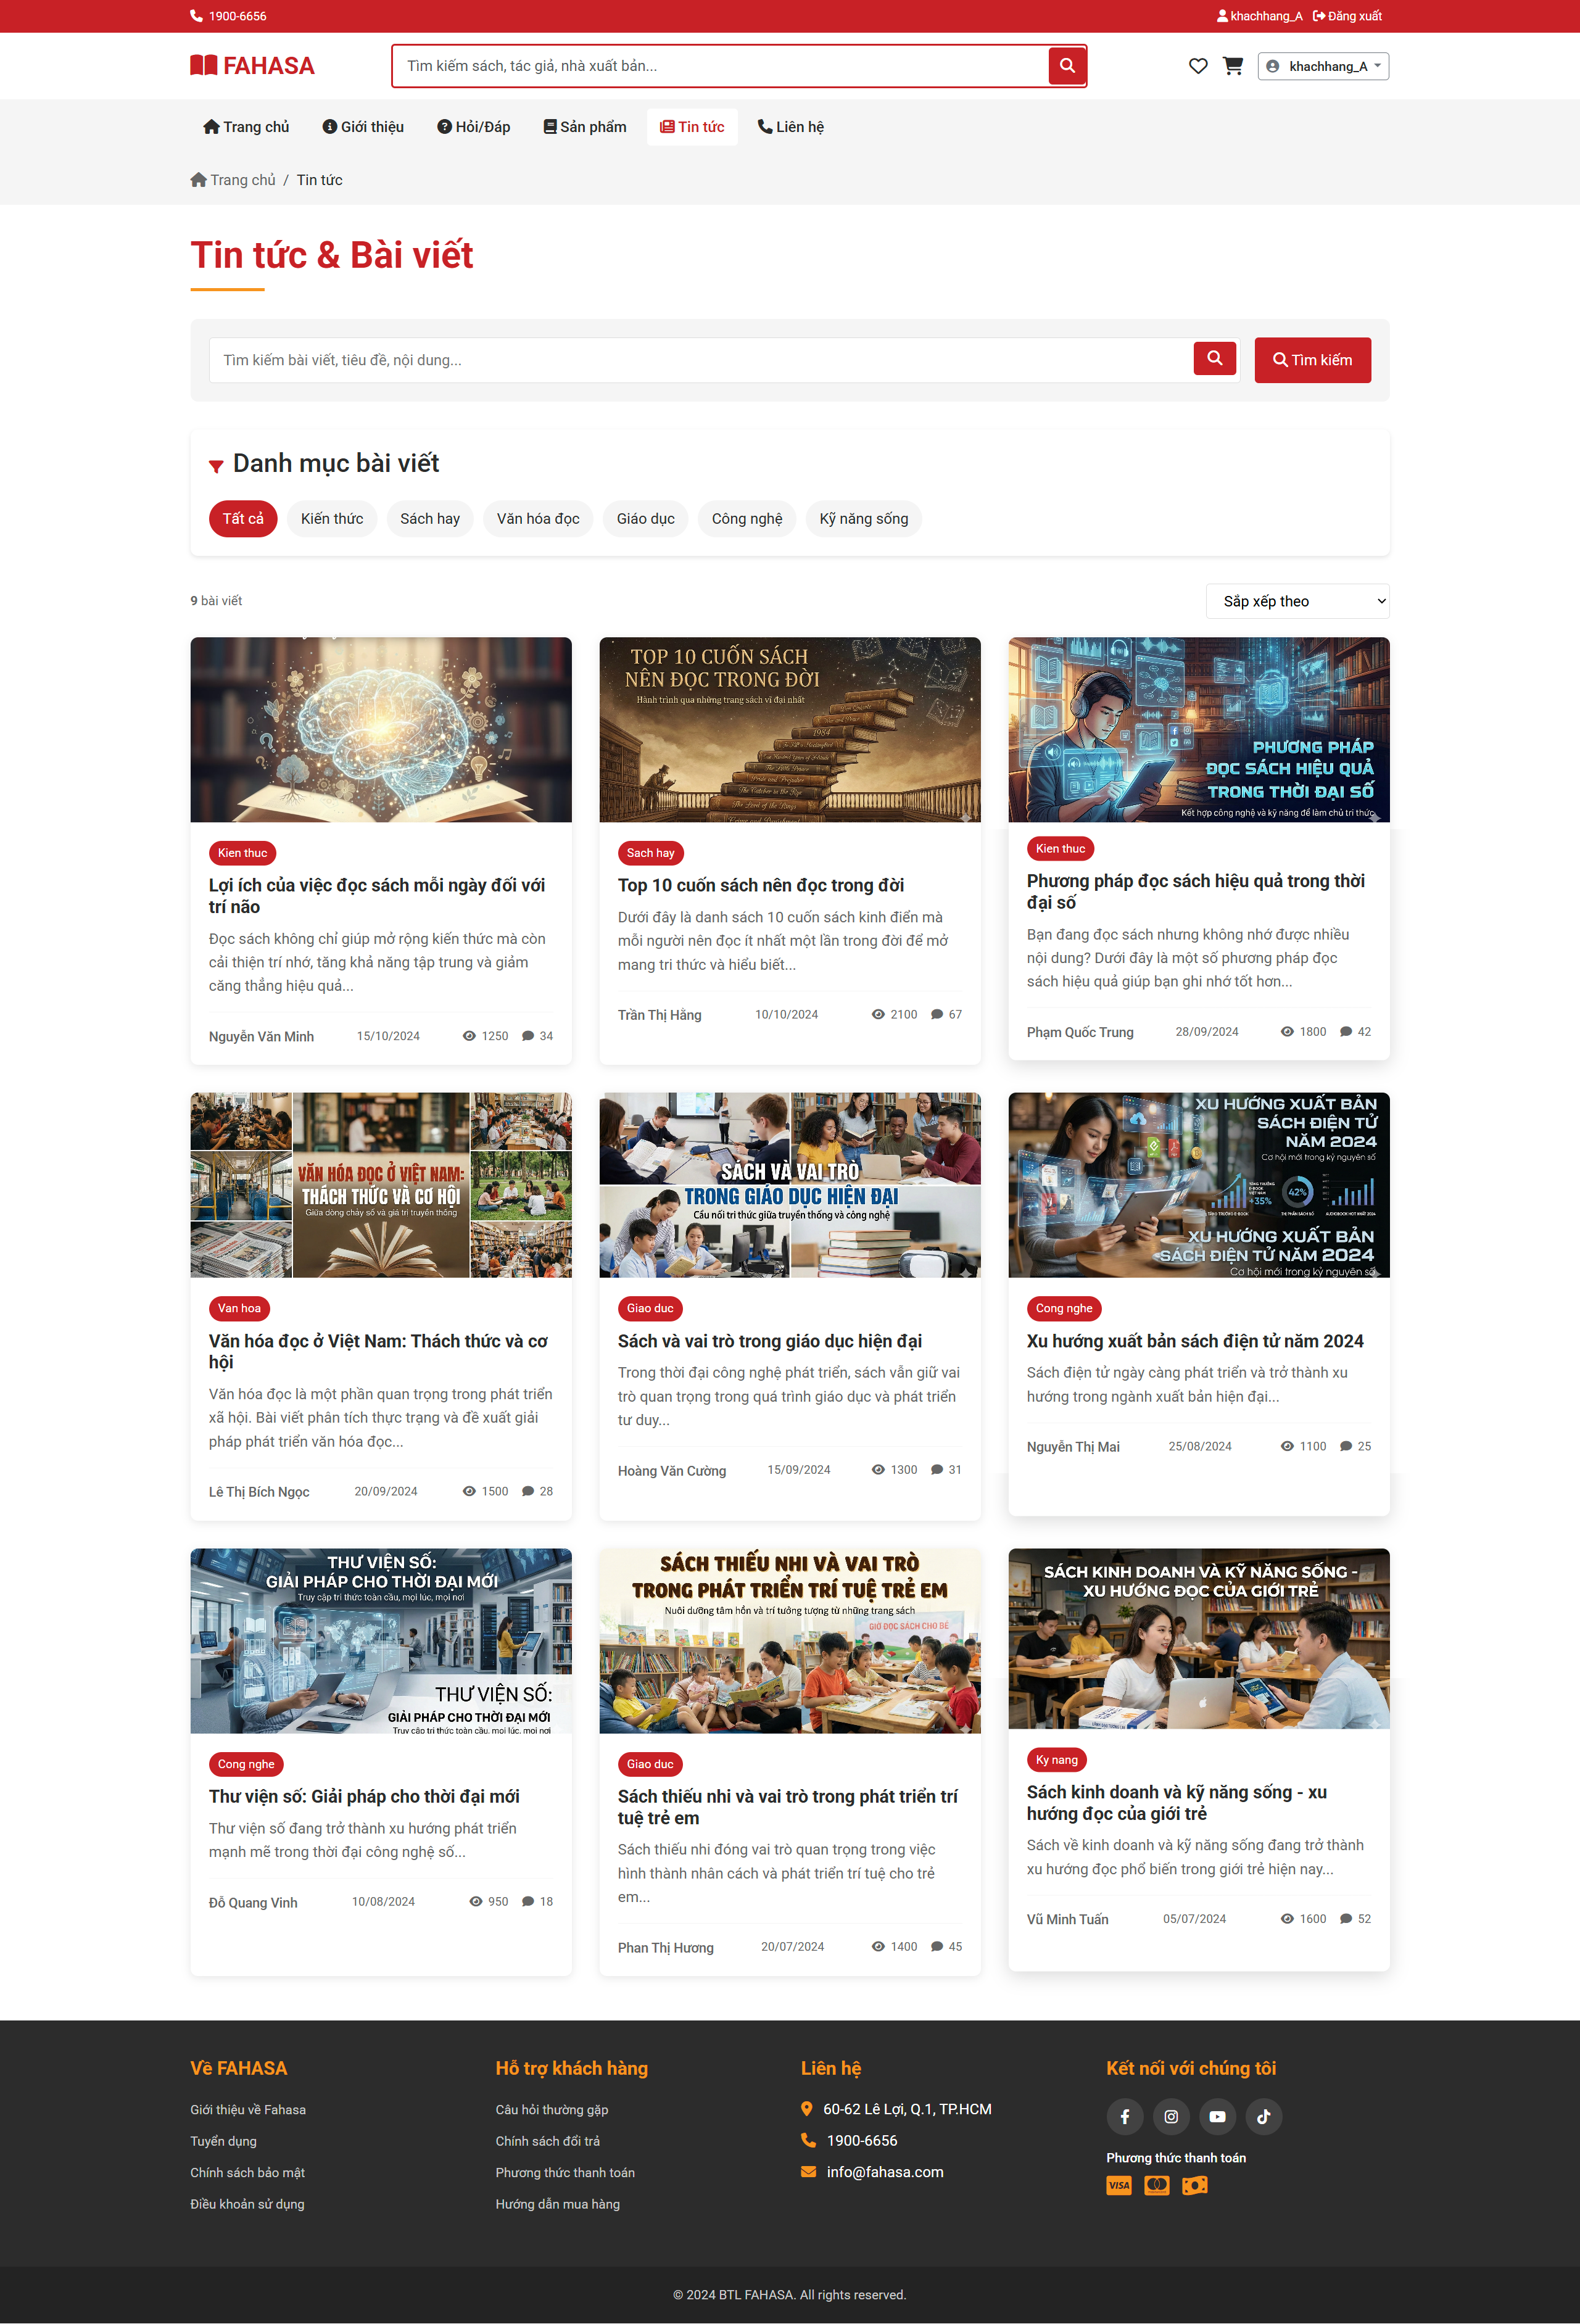
\includegraphics[width=0.6\textwidth]{Images/news_page.png}
\caption{Trang tin tức}
\label{fig:news}
\end{figure}

\subsubsection{Chi tiết bài viết}

Nội dung đầy đủ của bài viết, có phần bình luận:

\begin{figure}[H]
\centering
\includegraphics[width=0.6\textwidth]{Images/news_detail_page.png}
\caption{Trang chi tiết bài viết}
\label{fig:news-detail}
\end{figure}

% ------------------------------------------
\subsection{Các trang khác}

\subsubsection{Trang giới thiệu}

Giới thiệu về công ty Fahasa Clone:

\begin{figure}[H]
\centering
\includegraphics[width=0.6\textwidth]{Images/about_page.png}
\caption{Trang giới thiệu}
\label{fig:about}
\end{figure}

\subsubsection{Trang hỏi đáp}

FAQ - Câu hỏi thường gặp:

\begin{figure}[H]
\centering
\includegraphics[width=0.6\textwidth]{Images/qa_page.png}
\caption{Trang hỏi đáp}
\label{fig:qa}
\end{figure}

\subsubsection{Trang liên hệ}

Form liên hệ và thông tin công ty:

\begin{figure}[H]
\centering
\includegraphics[width=0.7\textwidth]{Images/contact_page.png}
\caption{Trang liên hệ}
\label{fig:contact}
\end{figure}

Giao diện Admin:

\begin{figure}[H]
\centering
\includegraphics[width=0.7\textwidth]{Images/dashboard_admin.jpg}
\caption{Trang Dashboard Admin}
\label{fig:dashboard_admin}
\end{figure}

\begin{figure}[H]
\centering
\includegraphics[width=0.7\textwidth]{Images/products_admin.jpg}
\caption{Trang Products Admin}
\label{fig:products_admin}
\end{figure}

\begin{figure}[H]
\centering
\includegraphics[width=0.7\textwidth]{Images/news_admin.jpg}
\caption{Trang Tin tức Admin}
\label{fig:news_admin}
\end{figure}

\begin{figure}[H]
\centering
\includegraphics[width=0.7\textwidth]{Images/contacts_admin.jpg}
\caption{Trang Contacts Admin}
\label{fig:contacts_admin}
\end{figure}

% ------------------------------------------
\subsection{Code snippets quan trọng}

\subsubsection{Router - App.php}

\begin{lstlisting}[style=phpstyle, caption=Core Router xử lý URL]
<?php
class App {
    protected $controller = 'HomeController';
    protected $method = 'index';
    protected $params = [];
    
    public function __construct() {
        $url = $this->parseUrl();
        
        // Load controller
        if(file_exists('../app/controllers/' . $url[0] . 'Controller.php')) {
            $this->controller = $url[0] . 'Controller';
            unset($url[0]);
        }
        
        require_once '../app/controllers/' . $this->controller . '.php';
        $this->controller = new $this->controller;
        
        // Call method
        if(isset($url[1]) && method_exists($this->controller, $url[1])) {
            $this->method = $url[1];
            unset($url[1]);
        }
        
        $this->params = $url ? array_values($url) : [];
        call_user_func_array([$this->controller, $this->method], $this->params);
    }
}
?>
\end{lstlisting}

\subsubsection{CartController - Thêm vào giỏ hàng}

\begin{lstlisting}[style=phpstyle, caption=Xử lý thêm sản phẩm vào giỏ]
<?php
public function add($productId = null) {
    if (!$productId) {
        $this->redirect('product');
    }
    
    // Get product info
    $product = $this->getProductById($productId);
    
    if ($product) {
        // Initialize cart if not exists
        if (!isset($_SESSION['cart'])) {
            $_SESSION['cart'] = [];
        }
        
        // Add or update quantity
        if (isset($_SESSION['cart'][$productId])) {
            $_SESSION['cart'][$productId]['quantity']++;
        } else {
            $_SESSION['cart'][$productId] = [
                'product' => $product,
                'quantity' => 1
            ];
        }
    }
    
    $this->redirect('cart');
}
?>
\end{lstlisting}

\subsubsection{JavaScript - Update Cart Quantity}

\begin{lstlisting}[style=jsstyle, caption=JavaScript xử lý tăng/giảm số lượng]
function updateQuantity(productId, action) {
    const input = document.querySelector(`#qty-${productId}`);
    let qty = parseInt(input.value);
    
    if (action === 'increase') {
        qty++;
    } else if (action === 'decrease' && qty > 1) {
        qty--;
    }
    
    input.value = qty;
    
    // Update via AJAX
    fetch(`/cart/update/${productId}/${qty}`, {
        method: 'POST'
    }).then(response => {
        updateCartTotal();
    });
}
\end{lstlisting}
